\documentclass[11pt,a4paper]{article}
%==============================================================================
%  Multi-Agent Systems & Agentic AI -- Practical Examination
%  SINGLE-FILE report scaffold covering the WHOLE submission:
%    Part I.1-I.3  -- practical GRPO write-up      (50 marks, <= 3 pages)
%    Part I.4      -- GRPO theory, LaTeX           (40 marks, no page limit)
%    Part II       -- adaptive planning critique   (30 marks, <= 2 pages
%                                                    EXCLUDING workflow diagram)
%  Final mark = (I.1-I.3 + I.4 + II) / 120.
%
%  This is a SCAFFOLD: structure + numbered given equations + "% TODO" answer
%  prompts only. Do not paste answers -- the report is individual and in your
%  own words (see ../CLAUDE.md and the spec docs/exam_2026_v2_questions.pdf).
%
%  FORMATTING IS A HARD REQUIREMENT -- do NOT change it to gain space:
%    A4 paper, 11pt body font, single column, margins >= 2cm, single line
%    spacing. Shrinking the font, margins, or line spacing to evade a page
%    limit is treated as over-length by the markers. The page limits are
%    counted EXCLUDING references and appendix; Part II's limit also excludes
%    the workflow diagram.
%
%  CLICKABLE LINKS ARE REQUIRED: every URL (GitLab repo, W&B run, dataset,
%  paper, cmbagent_lg commit) must be a clickable hyperlink -- use
%  \href{URL}{text} or \url{URL} (hyperref is loaded below).
%==============================================================================
\usepackage[a4paper,margin=2cm]{geometry}   % >= 2cm margins (required minimum)
\usepackage[T1]{fontenc}
\usepackage[utf8]{inputenc}
\usepackage{lmodern}
\usepackage{amsmath,amssymb}
\usepackage{graphicx}
\usepackage{booktabs}
\usepackage{caption}
\usepackage[numbers,sort&compress]{natbib}
\usepackage{xcolor}
\usepackage[colorlinks=true,allcolors=blue]{hyperref}
\usepackage{url}

\graphicspath{{figures/}}
% Single line spacing is the LaTeX default -- do NOT add \setstretch/\doublespacing.

\title{\vspace{-1.5em}Multi-Agent Systems \& Agentic AI --- Practical Examination\\[4pt]
       \large Part~I: GRPO finetuning of Gemma~3 on a TPU (Sections~I.1--I.4)\\
       \large Part~II: Adaptive planning in \texttt{cmbagent\_lg}}
\author{Sicheng Ma \\ \texttt{[CRSid / college]}}   % TODO: fill in CRSid and college
\date{\today}

\begin{document}
\maketitle
\vspace{-1.5em}

%------------------------------------------------------------------------------
% REQUIRED title-page metadata: team members, ownership statement, and links.
% The marker uses the ownership statement to attribute jointly-owned experiments.
% NOTE: Part I.4 (theory) and Part II are STRICTLY INDIVIDUAL -- only the
% practical sections I.1-I.3 describe shared team work.
%------------------------------------------------------------------------------
\noindent\textbf{Team members:} Sicheng Ma (author), \textit{[teammate name(s)]}.\\
\textbf{Jointly-owned experiments (I.1--I.3 only):} \textit{[state which runs / plots are shared with teammates; everything else, and all of I.4 and Part~II, is your own individual work]}.\\
\textbf{Code (GitLab):} \url{https://gitlab.com/USER/REPO}\quad % TODO: replace with your GitLab repo
\textbf{W\&B:} \url{https://wandb.ai/ENTITY/PROJECT}\\           % TODO: replace with your W&B run/project
\textbf{Baseline:} tpu-2026 @ \href{https://github.com/borisbolliet/tpu-2026/tree/324abbe4b4e229ea812223856393547db4fbb53e}{\texttt{324abbe}}.\quad
\textbf{Part~II study target:} \texttt{cmbagent\_lg} @ \href{https://github.com/borisbolliet/cmbagent_lg/tree/adaptive-planning}{\texttt{adaptive-planning}}. % TODO: pin the exact commit you studied

\vspace{0.5em}\hrule\vspace{0.6em}

% ============================================================================
%  PART I -- GRPO FINETUNING OF GEMMA 3 ON A TPU
%  Practical sections I.1-I.3 share a 3-page limit (excl. refs/appendix);
%  the theory section I.4 has no page limit but must be clear and concise.
% ============================================================================

% ----------------------------------------------------------------------------
%  I.1  Reproducing the baseline (10 marks)
%  Run scripts/train.py end-to-end on the v6e-1 with the default config.py,
%  then run scripts/evaluate.py on the resulting checkpoint.
% ----------------------------------------------------------------------------
\section{Reproducing the baseline}
\label{sec:reproduce}

% TODO (i): exact commit you ran, wall-clock time, and number of GRPO steps
% actually completed (default target MAX_STEPS = 3364).
\paragraph{Run provenance.}
\textit{TODO: exact commit (baseline \texttt{324abbe} plus any of your own commits on top), wall-clock time of the run, and GRPO steps actually completed (default \texttt{MAX\_STEPS}$=3364$).}

% TODO (ii): GSM8K accuracy of (a) the BASE model gemma-3-1b-it and (b) the
% LoRA-finetuned checkpoint, on a clearly-stated held-out split with a fixed
% seed. evaluate.py --preset greedy gives a deterministic number.
\paragraph{Held-out accuracy (base vs.\ LoRA).}
Held-out split: \textit{TODO (e.g.\ GSM8K test, $N$ prompts, fixed seed, \texttt{evaluate.py --preset greedy})}.
\begin{table}[h]
  \centering
  \caption{GSM8K accuracy: base \texttt{gemma-3-1b-it} vs.\ the baseline LoRA checkpoint (held-out split, greedy decoding, fixed seed). \emph{TODO: fill in.}}
  \label{tab:baseline-acc}
  \begin{tabular}{lccc}
    \toprule
    Model & Exact-match (\%) & Within $\pm10\%$ (\%) & Format acc.\ (\%) \\
    \midrule
    Base \texttt{gemma-3-1b-it}            & TODO & TODO & TODO \\
    Baseline LoRA (step \textit{TODO})     & TODO & TODO & TODO \\
    \bottomrule
  \end{tabular}
\end{table}

% TODO (iii): baseline training curve (mean reward r-bar vs GRPO step) and the
% KL divergence KL(pi_theta || pi_ref) over training.
\paragraph{Training curves.}
\begin{figure}[h]
  \centering
  % 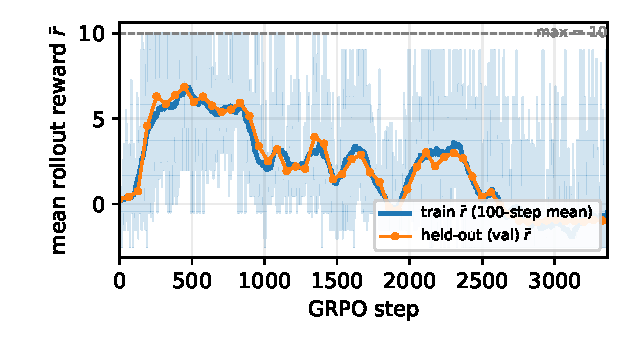
\includegraphics[width=0.48\textwidth]{baseline_reward.pdf}\hfill
  % 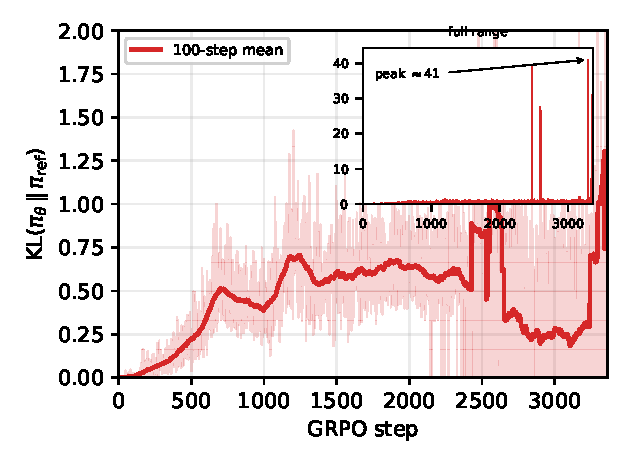
\includegraphics[width=0.48\textwidth]{baseline_kl.pdf}
  \caption{Baseline mean reward $\bar r$ (left) and $\mathrm{KL}(\pi_\theta\,\|\,\pi_{\mathrm{ref}})$ (right) vs.\ GRPO step. \emph{TODO: export from W\&B / TensorBoard into \texttt{figures/}.}}
  \label{fig:baseline-curves}
\end{figure}

% TODO: if anything did not run as-shipped on your hardware, document the fix
% here. Known environment-specific spots: run_tmux.sh hardcodes REPO/VENV paths;
% config.py W&B entity/project point at another account.
\paragraph{Baseline patches.}
\textit{TODO: document any change required to run the baseline as-shipped (e.g.\ the hardcoded \texttt{REPO}/\texttt{VENV} paths in \texttt{run\_tmux.sh}, or the \texttt{WANDB\_ENTITY}/\texttt{WANDB\_PROJECT} in \texttt{config.py}), or state ``none required''.}

% ----------------------------------------------------------------------------
%  I.2  Understanding the baseline (10 marks) -- at most ONE page, in your own
%  words. Map the baseline onto the formal objects defined in the lectures.
% ----------------------------------------------------------------------------
\section{Understanding the baseline}
\label{sec:understand}

% TODO (a): what plays the role of pi_theta, pi_old, pi_ref in the LoRA setup,
% and which of them carries trainable parameters?
\paragraph{(a) $\pi_\theta$, $\pi_{\mathrm{old}}$, $\pi_{\mathrm{ref}}$ in the LoRA setup.}
\textit{TODO (in your own words): identify each policy in the code --- frozen base $W_0$ plus low-rank adapters; see \texttt{scripts/model.py} and \texttt{config.py} (\texttt{RANK}, \texttt{ALPHA}) --- and state which one carries trainable parameters.}

% TODO (b): group size K in config.py, and which advantage estimator Tunix
% uses -- standard group baseline or leave-one-out?
\paragraph{(b) Group size $K$ and the advantage estimator.}
\textit{TODO: $K=2$ (\texttt{NUM\_GENERATIONS} in \texttt{config.py}); state whether Tunix's $\hat A_i$ uses the standard group mean/std baseline or the leave-one-out variant (check the Tunix GRPO implementation).}

% TODO (c): in rewards.py, which terms are shaping rewards and which is the
% "true" correctness reward? In terms of within-group reward variance sigma_r,
% what happens early in training with the correctness reward alone?
\paragraph{(c) Shaping vs.\ correctness rewards and $\sigma_r$.}
\textit{TODO: classify the four functions in \texttt{scripts/rewards.py} (exact / approximate format matching, \texttt{check\_answer}, \texttt{check\_numbers}); explain why correctness alone makes $\sigma_r\!\to\!0$ early (all-zero groups give degenerate $\hat A_i=(r_i-\bar r)/\sigma_r$) and how shaping rewards restore signal.}

% TODO (d): where is the clipped (PPO-style) surrogate implemented in Tunix,
% and what does the clip range epsilon correspond to in config.py? Note any
% deviation from the lecture form (e.g. per-token vs per-sequence ratio).
\paragraph{(d) The clipped surrogate and $\varepsilon$.}
\textit{TODO: locate the clipped-surrogate site in Tunix; $\varepsilon=0.2$ (\texttt{EPSILON}); note whether the ratio $\rho$ is applied per-token or per-sequence relative to the lecture form.}

% ----------------------------------------------------------------------------
%  I.3  Improving on the baseline (30 marks)
%  At least one PRINCIPLED, theory-motivated modification + a CONTROLLED
%  comparison. Expect >= 3 complete training runs total (baseline + 2 more),
%  with the same data, eval split, and total (or normalised-per-step) compute.
% ----------------------------------------------------------------------------
\section{Improving on the baseline}
\label{sec:improve}

% TODO: motivate the modification IN WRITING, grounded in lecture theory.
% Acceptable directions (not exhaustive):
%   - Algorithmic: leave-one-out advantage; sweep K and check Var(A_hat); change
%     beta/epsilon and report KL drift; reference-KL penalty on/off.
%   - Reward: remove/reweight a shaping term; add a length penalty; strict format.
%   - Data/curriculum: filter or reorder GSM8K; mix in a second math source.
%   - Optimisation/capacity: LoRA rank, learning rate, schedule, generation
%     length -- trade-off in KL budget vs effective sample size.
\paragraph{Motivation.}
\textit{TODO: name the modification and justify it from the theory in one short paragraph.}

\paragraph{Controlled comparison.}
\textit{TODO: state what is held fixed (data, eval split, total/normalised compute, seeds) and what changes.}

% TODO (a): table comparing base model, baseline GRPO checkpoint, and your
% improved checkpoint(s) on held-out GSM8K, WITH seeds and a measure of
% uncertainty (second seed or bootstrap CI over the eval prompts).
\begin{table}[h]
  \centering
  \caption{Held-out GSM8K: base vs.\ baseline vs.\ improved, with seeds and a measure of uncertainty (second seed / bootstrap CI). \emph{TODO.}}
  \label{tab:improve-acc}
  \begin{tabular}{llccc}
    \toprule
    Run & Change & Acc.\ (\%) $\pm$ CI & Mean reward & Final KL \\
    \midrule
    Base \texttt{gemma-3-1b-it}     & ---                        & TODO & --- & --- \\
    Baseline GRPO                   & default \texttt{config.py} & TODO & TODO & TODO \\
    Variant A                       & \textit{TODO}              & TODO & TODO & TODO \\
    Variant B (2nd seed / 2nd mod)  & \textit{TODO}              & TODO & TODO & TODO \\
    \bottomrule
  \end{tabular}
\end{table}

% TODO (b): training curves of mean reward AND KL for the baseline and your
% variants on a SINGLE set of axes.
\begin{figure}[h]
  \centering
  % \includegraphics[width=0.48\textwidth]{improve_reward.pdf}\hfill
  % \includegraphics[width=0.48\textwidth]{improve_kl.pdf}
  \caption{Mean reward (left) and KL (right) for the baseline and your variants on shared axes. \emph{TODO.}}
  \label{fig:improve-curves}
\end{figure}

% TODO (c): ONE diagnostic plot addressing a known GRPO failure mode -- e.g.
% distribution of A_hat_i over training, fraction of degenerate groups (all K
% rewards equal), response length / entropy of pi_theta over time, or KL vs
% task accuracy.
\begin{figure}[h]
  \centering
  % \includegraphics[width=0.6\textwidth]{diagnostic.pdf}
  \caption{Diagnostic for a known GRPO failure mode (e.g.\ fraction of degenerate groups where all $K$ rewards are equal, or the $\hat A_i$ distribution over training). \emph{TODO.}}
  \label{fig:diagnostic}
\end{figure}

% TODO (d): discuss how your empirical findings connect to the lecture theory,
% INCLUDING any prediction you contradicted. Honest negative results are in scope.
\paragraph{Discussion.}
\textit{TODO: connect your findings to the theory; report any contradicted prediction (``we tried X, theory predicted Y, we observed Z'').}

% ============================================================================
%  I.4  GRPO THEORY -- written questions (40 marks)
%  Individual. No page limit, but verbosity is penalised: be clear and concise.
%  MUST be typeset in LaTeX with amsmath; number any equation you refer back to.
%  Below: the GIVEN setup is restated (numbered) so you can cite it; each
%  sub-part has a "% TODO" answer slot. Write the derivations in your own words.
% ============================================================================
\clearpage
\section{GRPO theory}
\label{sec:theory}

% ---- Q1 -------------------------------------------------------------------
\subsection{Variance of the group-normalised gradient estimator}
\label{sec:theory-q1}
For a fixed prompt $q$ and $K\ge 2$ responses $a_1,\dots,a_K$ (treated as fixed),
let $r_1,\dots,r_K$ be i.i.d.\ rewards with mean $\mu$ and variance $\sigma^2$.
Define the group mean and normalised advantage
\begin{equation}
  \bar r \;=\; \frac{1}{K}\sum_{i=1}^{K} r_i,
  \qquad
  \hat A_i \;=\; \frac{r_i-\bar r}{\sigma_r},
  \label{eq:q1-adv}
\end{equation}
treating $\sigma_r=\sigma$ as a known constant. With deterministic score vectors
$h_i=\nabla_\theta\log\pi_\theta(a_i\mid q)\in\mathbb{R}^d$, define
\begin{equation}
  X_i \;=\; h_i\,\hat A_i,
  \qquad
  \hat g \;=\; \frac{1}{K}\sum_{i=1}^{K} X_i \;\in\; \mathbb{R}^d.
  \label{eq:q1-ghat}
\end{equation}

\paragraph{(i) $\mathbb{E}[X_i]$, $\mathbb{E}[\hat g]$, and why the true gradient need not vanish. \hfill\textnormal{[2]}}
\textit{TODO: compute $\mathbb{E}[X_i]$ and hence $\mathbb{E}[\hat g]$; in $\le 2$ sentences explain why $\mathbb{E}[\hat g]=0$ here does \emph{not} mean the underlying policy gradient vanishes (responses are held fixed; the expectation over rewards differs from the expectation over the sampling distribution).}

\paragraph{(ii) $\mathrm{Cov}(X_i,X_j)$ for $i\neq j$. \hfill\textnormal{[6]}}
\textit{TODO: identify the shared random term that couples the $X_i$ (the common $\bar r$); compute $\mathrm{Cov}(X_i,X_j)$ in terms of the outer product $h_i h_j^{\top}$ and the moments of $r$; state the sign of the result and explain intuitively why it arises.}

\paragraph{(iii) $\mathrm{Var}(\hat g)$ and the effective sample size $K_{\mathrm{eff}}$. \hfill\textnormal{[7]}}
\textit{TODO: compute $\mathrm{Var}(\hat g)\in\mathbb{R}^{d\times d}$; compare with the naive i.i.d.\ expectation $\tfrac{1}{K}\mathrm{Var}(X_1)$; use the discrepancy to \emph{define} an effective sample size $K_{\mathrm{eff}}$, give an explicit expression in terms of $\mathrm{Var}(X_1)$, and comment on large $K$ and on the case where all $h_i$ are aligned.}

% ---- Q2 -------------------------------------------------------------------
\subsection{KL-regularised policy improvement and the clipped surrogate}
\label{sec:theory-q2}
Let $\mathcal{A}$ be an action space and $\pi_t$ the policy at iteration $t$, with
a fixed advantage function $A_t:\mathcal{A}\to\mathbb{R}$. For policies $p,q$,
$\mathrm{KL}(p\|q)=\sum_a p(a)\log\frac{p(a)}{q(a)}$ (with $0\log 0=0$).
Consider the regularised update
\begin{equation}
  \pi_{t+1} \;=\; \arg\max_{\pi}\;
  \Bigl\{\, \mathbb{E}_{a\sim\pi}[A_t(a)] \;-\; \tfrac{1}{\eta}\,\mathrm{KL}(\pi\|\pi_t) \,\Bigr\},
  \qquad \eta>0.
  \label{eq:q2-update}
\end{equation}

\paragraph{(i) Unique optimiser of \eqref{eq:q2-update} and the role of $\eta$. \hfill\textnormal{[3]}}
\textit{TODO: derive the unique maximiser (softmax tilt of $\pi_t$ by $\eta A_t$) and explain $\eta$ as a step-size parameter.}

\paragraph{(ii) Monotone improvement and where it fails. \hfill\textnormal{[5]}}
\textit{TODO: with $J(\pi)=\mathbb{E}_{a\sim\pi}[A^{\pi_t}(a)]$ and exact advantage $A_t=A^{\pi_t}$, show \eqref{eq:q2-update} guarantees $J(\pi_{t+1})\ge J(\pi_t)$; identify one practical condition under which this guarantee fails for a neural-network policy (e.g.\ stale / estimated advantage, function-approximation error, finite-sample KL).}

\paragraph{(iii) Trust region of the clipped surrogate vs.\ the KL constraint. \hfill\textnormal{[2]}}
With $\pi_{\mathrm{old}}=\pi_t$, $a_t\sim\pi_{\mathrm{old}}(\cdot\mid q)$,
\begin{equation}
  \rho_t(\theta)=\frac{\pi_\theta(a_t\mid q)}{\pi_{\mathrm{old}}(a_t\mid q)},
  \qquad
  J^{\mathrm{clip}}(\theta)=\mathbb{E}_t\!\Bigl[\min\bigl(\rho_t(\theta)\hat A_t,\;
  \mathrm{clip}(\rho_t(\theta),1-\varepsilon,1+\varepsilon)\hat A_t\bigr)\Bigr].
  \label{eq:q2-clip}
\end{equation}
\textit{TODO: describe the per-sample trust region the clip induces, contrast it with the single joint constraint $\mathrm{KL}(\pi_\theta(\cdot\mid q)\|\pi_{\mathrm{old}}(\cdot\mid q))\le\delta$ implicit in \eqref{eq:q2-update}, and state at least one qualitative difference.}

% ---- Q3 -------------------------------------------------------------------
\subsection{Mixture-proposal sampling, importance correction, and weight collapse}
\label{sec:theory-q3}
Fix $q$ and a fixed sampling policy $\pi_{\mathrm{old}}(\cdot\mid q)$; let
$R(q,a)\in\mathbb{R}$ be a deterministic reward and
$V^{\pi}(q)=\mathbb{E}_{a\sim\pi(\cdot\mid q)}[R(q,a)]$. Standard GRPO draws
$a_1,\dots,a_K\stackrel{\mathrm{iid}}{\sim}\pi_{\mathrm{old}}$, sets $r_i=R(q,a_i)$ and forms
\begin{equation}
  \hat g_{\mathrm{GRPO}} \;=\; \frac{1}{K}\sum_{i=1}^{K}\nabla_\theta\log\pi_\theta(a_i\mid q)\,\hat A_i,
  \qquad \hat A_i=\frac{r_i-\bar r}{\sigma_r}.
  \label{eq:q3-grpo}
\end{equation}
Consider instead the mixture proposal
\begin{equation}
  \pi_{\mathrm{mix}}(a\mid q) \;=\; (1-\alpha)\,\pi_{\mathrm{old}}(a\mid q) \;+\; \alpha\,\pi_{\mathrm{unif}}(a\mid q),
  \qquad \alpha\in[0,1),
  \label{eq:q3-mix}
\end{equation}
with $\pi_{\mathrm{unif}}$ uniform over responses.

\paragraph{(i) Importance-corrected estimator $\hat g_{\mathrm{mix}}$. \hfill\textnormal{[3]}}
\textit{TODO: derive $\hat g_{\mathrm{mix}}$ using samples from $\pi_{\mathrm{mix}}$ and give the explicit importance weight $w_i=\pi_{\mathrm{old}}(a_i\mid q)/\pi_{\mathrm{mix}}(a_i\mid q)$.}

\paragraph{(ii) Limit $\alpha\to0$. \hfill\textnormal{[1]}}
\textit{TODO: verify $\hat g_{\mathrm{mix}}\to\hat g_{\mathrm{GRPO}}$ for the same realised actions as $\alpha\to0$.}

\paragraph{(iii) The shifted group mean. \hfill\textnormal{[1+2]}}
\textit{TODO (a): express $V^{\pi_{\mathrm{mix}}}(q)$ in terms of $V^{\pi_{\mathrm{old}}}(q)$ and $V^{\pi_{\mathrm{unif}}}(q)$. TODO (b): determine whether the weights $w_i$ alone correct for the baseline shift, and derive the reweighted advantage that keeps $\hat g_{\mathrm{mix}}$ unbiased for the policy gradient under $\pi_{\mathrm{old}}$.}

\paragraph{(iv) Variance comparison. \hfill\textnormal{[4]}}
\textit{TODO: compare $\mathrm{Var}(\hat g_{\mathrm{mix}})$ with $\mathrm{Var}(\hat g_{\mathrm{GRPO}})$ at fixed $K$; give one condition on $R$ under which mixing \emph{increases} the variance and a different one under which it \emph{decreases} it, with a brief argument for each.}

\paragraph{(v) Weight collapse for long responses. \hfill\textnormal{[2+2]}}
Assume the per-token ratio $\pi_{\mathrm{old}}(a_{i,t}\mid q,a_{i,<t})/\pi_{\mathrm{mix}}(a_{i,t}\mid q,a_{i,<t})=c$ is constant, so the full-response weight is $w_i=c^{T}$ for $T$ tokens.
\textit{TODO (a): describe $w_i$ as $T\to\infty$ and explain in one sentence why $c<1$ is typical when $\alpha>0$. TODO (b): explain why this ``weight collapse'' makes $\hat g_{\mathrm{mix}}$ unreliable for long responses, and propose one concrete fix (to $\pi_{\mathrm{mix}}$ or the weighting) stating what it trades off.}

% ============================================================================
%  PART II -- ADAPTIVE PLANNING IN cmbagent_lg (individual, 30 marks)
%  At most 2 pages EXCLUDING the workflow diagram. Read, diagram, and critique
%  the adaptive-planning branch -- you are NOT asked to build a system.
%  Frozen study target (pin the exact commit on the title page):
%    https://github.com/borisbolliet/cmbagent_lg/tree/adaptive-planning
%  Study the planning/ and deep_research/ modules of cmbagent_lg/adaptive_planning.
% ============================================================================
\clearpage
\section*{Part~II --- Adaptive planning in \texttt{cmbagent\_lg}}
\addcontentsline{toc}{section}{Part II --- Adaptive planning in cmbagent\_lg}
\label{sec:partii}

% ---- II.1 ------------------------------------------------------------------
\subsection*{II.1\quad Workflow diagram (12 marks)}
\label{sec:partii-diagram}
% The workflow diagram does NOT count towards the 2-page limit. Produce it as a
% LangGraph-style node/edge diagram -- either an \includegraphics figure
% (export from a drawing tool) or a TikZ picture -- showing nodes, edges,
% conditional routing, and the state threaded between nodes.
\begin{figure}[h]
  \centering
  % \includegraphics[width=\textwidth]{cmbagent_lg_workflow.pdf}  % TODO: export your diagram
  \caption{Adaptive-planning workflow of \texttt{cmbagent\_lg} (\texttt{adaptive-planning} branch): LangGraph nodes (planner, plan-reviewer, control loop, adaptive-review), edges, conditional routing, and the state object threaded between nodes. \emph{TODO: replace with your diagram --- this figure does not count towards the 2-page limit.}}
  \label{fig:partii-workflow}
\end{figure}

\paragraph{Walkthrough.}
\textit{TODO (at most half a page): make explicit what triggers a plan revision, what part of the plan may change, what is held fixed across a revision, and how the loop is guaranteed to terminate.}

% ---- II.2 ------------------------------------------------------------------
\subsection*{II.2\quad Problems (9 marks)}
\label{sec:partii-problems}
\textit{TODO: identify and \emph{argue} (not merely assert) the most significant problems, limitations, or failure modes of the implementation, each grounded in the lecture material on planning and closed-loop control (e.g.\ open- vs closed-loop, plan staleness, oscillation / non-termination, observability of execution feedback, reviewer-planner coupling).}

% ---- II.3 ------------------------------------------------------------------
\subsection*{II.3\quad Proposed improvements (9 marks)}
\label{sec:partii-improvements}
\textit{TODO: for each problem raised in II.2, propose a concrete, justified improvement --- state what it changes, why it addresses the problem, and what it trades off (extra cost, added latency, new failure modes). Each proposal must be specific enough that someone could implement it.}

% ============================================================================
%  REFERENCES (do not count towards any page limit)
% ============================================================================
\bibliographystyle{plainnat}
\bibliography{references}

% ============================================================================
%  APPENDIX (optional; does not count towards page limits, but must not contain
%  material essential to the marking). Add \appendix and \section{...} here if
%  you need extra figures or derivation details.
% ============================================================================

\end{document}
